\documentclass{article}
\usepackage{graphicx}

\title{Implementation}
\begin{document}
    \maketitle

    A system was developed to perform two way conversion from natural language to actions, and from actions to natural language. The system uses Conceptual Dependancy representations of scenarios as intermediaries between natural language and physics situations.

    \section{Natural language to Actions}
    \begin{figure}[h]
        \begin{center}
            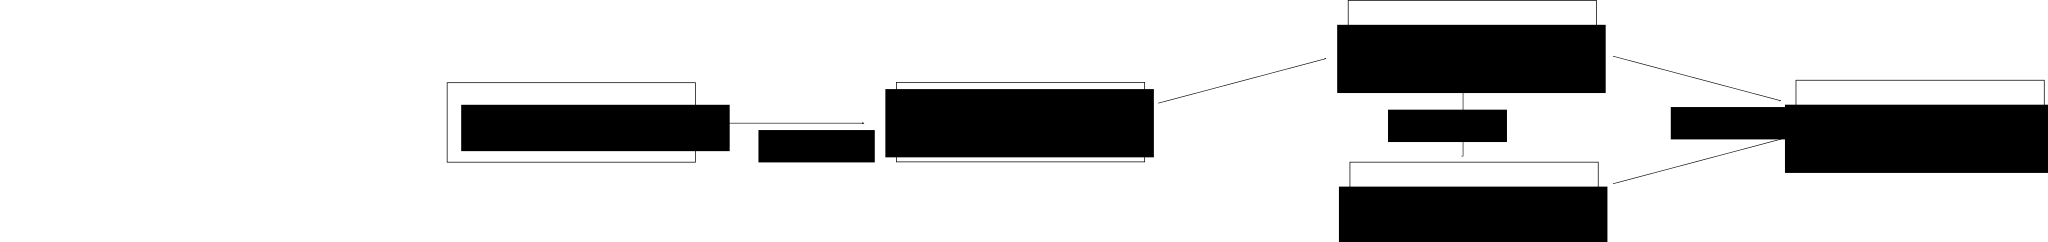
\includegraphics[width=300pt]{diagrams/verb-to-action-workflow.png}
        \end{center}
        \caption{The workflow for parsing an event expressed in natural lanuage into it's physical representation}
    \end{figure}

    The first step is parsing a natural language event into a predicate-argument structure relating subject and object. Each verb sense will have a definition in terms of conceptual dependencies- which CD primitive it corresponds to, which physical attribute it affects (e.g.~the `eject' verb indicates the object has been removed from inside the subject, meaning an `inside\_subject' attribute is assigned to that verb), and \emph{how} that attribute changes.

    Each verb definition will have a CD primitive assigned to it- each of these primitives will have it's own properties such as the attribute it affects, and any constraints on the subject/ object type. The verb definition is then merged with the primitive definition (there should be no contradictory fields). This merging allows sparser verb definitions, with some information already implicit in the primitive.

    An example of different verbs with the same primitive is `eject' and `emit'- both of these terms best correspond to the CD primitive ``EXPEL'', however they will generally be used for different kinds of materials. Eject will generally be used for solid structures being expelled from a larger one, whereas `emit' would generally be used for radiation or energy being expelled.

    In this case, the system can be guided to using the more suitable verb by applying a type constraint to the object of the verb (object being used in the logical sense). Constraints in existing natural language libraries aren't generally specific enough for these purposes, so a crude list of physics-specific constraint rules was built as a proof of concept.
    
    \section{Actions to Natural Language}
    \begin{figure}[h]
        \begin{center}        
            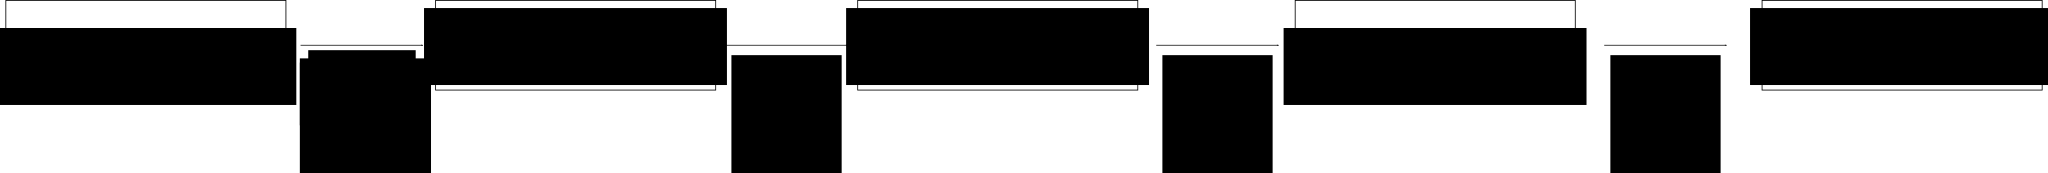
\includegraphics[width=300pt]{diagrams/action-to-verb-workflow.png}
        \end{center}
        \caption{The workflow for parsing an event expressed in natural lanuage into it's physical representation}
    \end{figure}

    Converting an event to it's Conceptual Dependencies and then into natural language uses much of the same infrastructure in reverse, with the additional aspect of an underlying physical simulation. This simulation reports notable `events' to the Manager unit, in terms of what attribute on an object was changed, and in what way.

    Primitives which contradict the information in the event are eliminated, thus restricting the candidate verbs to only those which are relevant. These are then filtered according to the remaining criteria (affected_attribute, attribute outcome, and any selectional restrictions).

    \section{Physics Simulation}
    \subsection{Recognition of physical events}


\end{document}